
\section{Measuring charge transport}

In this section the Hall measurement technique and analysis of the \ac{BSCO} samples is described. Transport measurements on superconductors have been performed for over a century now and was the technique by which superconductivity was first discovered. The relative technical simplicity of the measurements makes transport measurements highly appealing considering the wealth of information that can be extracted from a resistance curve.


\subsection{Experimental apparatus}

\subsubsection{Six probe technique}
\label{Sec:Exp:SixProbe}

For accurate measurement of voltage, and hence resistance, across a sample, two wires are not sufficient. The wires and contacts themselves have a resistance which is comparable or often larger than the resistance of the sample being measured. A solution to this problem is to instead supply the current for the voltage reading via one set of wires, and then take the voltage reading from another set meaning that a minimum of four wires and four contacts on the sample are required. To measure magnetoresistance we require the voltage wires to be placed upstream and downstream of the current contacts, to measure the Hall effect we require the wires to be placed transverse to the current. Moreover it is useful to be able to take two transport measurements on opposite sides of the sample so as to get an idea for the homogeneity of the sample and as well to provide some redundancy in case of breakage. Since the \ac{BSCO} samples that we studied were to have both measurements, six connection points were placed on each sample as shown in figure~\ref{Fig:Exp:BSCOSampleSchematic}.
\begin{figure}[htbp]
    \begin{center}
        \includegraphics[scale=1.1]{Chapter-ExperimentalTechnique/Figures/BSCOSampleSchematic/BSCOSampleSchematic}
        \caption{An example \ac{BSCO} crystal mounted on the quartz substrate. Voltage legs are labeled (a), (b), (c) and (d).}
        \label{Fig:Exp:BSCOSampleSchematic}
    \end{center}
\end{figure}
The connections were made with \unit{20}{\micro\metre} gold wire for the current and \unit{10}{\micro\metre} gold wire for the voltage leads and attached with DuPont 4929 conductive silver paint which dries at room temperature. As shown in the figure, the sample is raised from the quartz substrate so that when the temperature drops and the wires and sample thermally contract at low temperatures, there is some give so that the ensemble does not pull itself apart due to thermal contraction.

With the four voltage legs a variety of configurations can be achieved. Measuring across (a) and (b) is the magnetoresistance configuration, (a) and (c) is the Hall configuration. It is also possible to measure across (a) and (d) and provided the field is reversed from positive to negative, both the Hall and the magnetoresistance across the sample can be extracted.

Because the connections may not be exactly aligned and because the silver paint in practice tends to wet over the edge of the sample, magnetoresistance contributions may be found in the Hall configuration and vise-versa. For this reason it is generally advised to sweep both with a positive field to obtain $R_{\textrm{pos}}$ and a negative field to obtain $R_{\textrm{neg}}$ where $R$ is the resistance and separate the two out using the technique described in the analysis section.

Later as the samples have been measured many times and thermal cycling had caused the silver paint to become brittle, it was necessary to attach short, $\sim\unit{2}{\milli\metre}$, secondary gold wires to each of the contact pads using silver paint and then attach the probe flying leads to the end of these wires. When removing the samples from the probe, this allowed the joins to be immersed in solvent held in the tip of a pair of metal tweezers at a safe distance from the sample ensemble meaning the connection could be dissolved without flexing the contact pads unnecessarily. This was done for the later measurements in the \unit{16}{\tesla} `Polo' magnet where the minimisation of wire loops was not so important.

\subsubsection{\unit{16}{\tesla} `Polo' magnet}

The system informally referred to as the `Polo' magnet is a cryostat from Cryogenic Ltd. containing a \ac{VTI} refrigeration device that allows temperature from $\sim$\unit{1.4}{\kelvin} to room temperature to be achieved. The \ac{VTI} system is a vacuum sealed chamber in to which the sample probe is inserted and sealed at the top. This chamber is insulated from a bath of $^4$He in the main cryostat by a vacuum jacket. $^4$He is admitted into the \ac{VTI} chamber from the bath via an adjustable needle valve and is pumped through the chamber and over the sample by an external roughing pump. By almost closing off the needle valve entirely and applying a heater on the sample stage the full range of temperatures can be achieved. In practice, a couple of temperature ranges are defined which require different operational techniques and are specified in table~\ref{Table:Exp:PoloOperation}.
\begin{table}
    \begin{center}
           \caption{Operating the \ac{VTI} under various temperature regimes.}
        \begin{tabular}[htbp]{lp{7cm}}
\toprule
Temperature range & Practice \\
\midrule
\unit{1.4}{\kelvin} -- \unit{4.2}{\kelvin} & Fill \ac{VTI} chamber with helium, close off needle valve and adjust the pumping rate to tune the temperature. \\
\unit{4.2}{\kelvin} -- \unit{300}{\kelvin} & Empty the \ac{VTI} of helium and open the needle valve slightly, only pump a small amount and use the sample heater to set the temperature.  \\
\bottomrule
        \label{Table:Exp:PoloOperation}
        \end{tabular}
    \end{center}
\end{table}
The \ac{VTI} chamber itself has an electric heater which can be operated separately and is good for rapidly heating the system up to room temperature but is in general too coarse for measurements.

Heating is controlled by a Lakeshore 340 temperature controller with the sample stage heated from the heater output and the \ac{VTI} heater controlled from the analogue output which has been boosted via a custom built amplifier unit. Sample temperature is monitored by a Cernox mounted onto the sample stage and \ac{VTI} temperature from a thermometer mounted inside the \ac{VTI} chamber.

The sample stage can be rotated by an external stepper motor which is supplied from a custom power source. All the instruments mentioned are controlled from a custom PC running a Delphi program written by Dr. M. French which queues runs, records and displays data. Some calculated values based on the raw data values are generated by the software, however these were not configured with the appropriate inputs. For this reason the angle and the current fields should be ignored and instead determined from raw data.

For twin voltage measurements, two Stanford SR830 lock-in amplifiers were used with one supplying the current and measuring voltage and the second synchronised to the first and also measuring a voltage. The current supplied was supplied through a \unit{1}{\kilo\ohm} buffer resistor in order to approximate the supply to a current source\footnote{A current source can be approximated if ($R_{\textrm{sample}} + R_{\textrm{wires}}) << R_{\textrm{buffer}} $ at all $T$. The current is then given by $V_{\textrm{excitation}}/R_{\textrm{buffer}}$.}. The resulting voltages were passed through two passive Princeton Applied Research model 1900 low noise amplifiers set to $\times1000$ before measurement although the actual amplification for typical resistances of $10$--$100\Omega$ at \unit{33}{\hertz} is $\times 980$.

The sample probe has a rotating stage and so after aligning the sample roughly by eye, a shallow angle sweep in a low field, typically \unit{1}{\tesla}, was performed before each measurement to make sure the sample was positioned perpendicular to the field. Some samples have an anisotropy in the transport terms and in the case of the Hall component, the effective field drops with the cosine of the angle of misalignment.

The magnet is superconducting and has a limit of \unit{14}{\tesla} or \unit{16}{\tesla} when using the additional cooling of the Lambda plate. For this thesis the measurements were only taken to \unit{13}{\tesla} to minimise the risk of a quench. The field was ramped at \unit{1.4}{\tesla\per\minute}. The measurements presented in this thesis from the \unit{16}{\tesla} Polo magnet are all taken in the Hall configuration and are obtained by averaging both sets of contacts as described in the analysis section.

As of Feb 2012 it was determined using a Cu sample that a positive reading of the magnet power supply current (and field) with the leads wired up correctly (i.e. positive to positive, negative to negative) corresponds to the magnetic field, $B$, in the Polo magnet pointing upwards. This was verified with a magnetic compass.


\subsubsection{\acs{HFML} Nijmegen}

To access the normal state of the higher $T_c$ materials we require fields larger than the \unit{13}{\tesla} available in the Polo magnet at Bristol. The \acf{HFML} facility in Nijmegen has available a continuous field Bitter magnet which can reach \unit{33}{\tesla}. Data from Nijmegen in this thesis was taken in May 2010 by Dr. X. Xu, I. Mouzoupoulou, Dr. P. Rourke and Dr. A. McCollam.

The magnet used at the \ac{HFML} sweeps at a rate of typically \unit{3}{\tesla\per\minute} meaning the temperature can drift significantly. The necessary heating supply for temperature control was alternated between a Lakeshore 340 temperature controller which uses input from a Cernox thermometer and a PID algorithm to supply an appropriate current or a Keithley current source which supplies a fixed current. The current source was selected on a sweep-by-sweep basis depending on which gave more stable temperatures.  The analysis compensates for small drift using a simple correction described later. 

The samples were measured using Stanford SR830 lock-in amplifiers which were supplying via \unit{1}{\kilo\ohm} resistors with a \unit{10}{\ohm} shunt resistor. A \unit{1}{\volt} excitation voltage was used for all samples except for B00KOD1a and B16KOD1a where \unit{2}{\volt} excitation was used instead. The excitation frequency is set to one of the `magic' frequencies\footnote{Frequencies that do not fall near common sources of noise or their harmonics e.g. \unit{50}{\hertz} from mains supply.} which in this case were \unit{33}{\hertz}, \unit{77}{\hertz}, \unit{113}{\hertz} and \unit{123}{\hertz}.

Field is monitored using a calibrated Hall sensor mounted on the probe which is measured using another Stanford SR830 lock-in amplifier.

\subsubsection{\acs{LNCMI} Toulouse}

To obtain the highest fields we took measurements at the \acf{LNCMI} pulsed field facility in Toulouse over the course of two separate visits. Here large capacitor banks are discharged through liquid nitrogen cooled copper resistive magnets to achieve short (few tens of microseconds) but strong fields of up to \unit{60}{\tesla}. Pulses at the stronger end of the scale have more potential for damaging the magnet and take longer to cool down before the next pulse can be taken and so careful consideration is required to the magnitude of pulse undertaken. Typically the cooling time is around 15 to 30 minutes. The field is measured using a calibrated pick-up coil. The first trip took place in June 2009 and involved B. Arnold, Dr. P. Rourke, Dr. B. Vignolle and Prof. C. Proust. the second trip occurred in February 2010 and involved Dr. P. Rourke, Dr. J. F. Mercure, Prof. N. Hussey, Dr. B. Vignolle and Prof. C. Proust.

The results are recorded using a pair of Stanford SR830 lock-in amplifiers after passing through an active INA103 pre-amplifier set to a gain of $\times200$. The raw signal for the pulse duration is recorded and the lock-in in algorithm is post-processed in software to avoid wasted pulses due to incorrect settings. The driving current is supplied by the lock-in amplifier and unless otherwise noted is \unit{5}{\volt} through a \unit{1}{\kilo\ohm} resistor giving a current source of \unit{5}{\milli\ampere}. The driving frequency is typically very high to sample the data over the relatively short pulse time and for these experiments is typically \unit{60}{\kilo\hertz}. The data is streamed via an optical link along glass fibres (so the chamber remains electrically isolated for safety during a pulse) to an external PC.

Cooling down to $\sim \unit{1.4}{\kelvin}$ is possible by pumping on the helium in the magnet bath. Higher temperatures could be achieved by pumping out the exchange gas and heating via a Lakeshore 340 temperature controller. Although pulses are very short lived, there is a risk of the rapidly changing field inducing a current in the leads and sample which cause heating of the sample during the pulse. For this reason great care is taken to minimise current loops by minimising the non-twisted portion of the wires leading to the sample. Furthermore, the sample is physically jolted by the high field which can adversely affect the data, for this reason, vacuum grease is carefully applied to the sample ensemble to reduce movement.

For the first Toulouse visit, the measurements were taken in the magnetoresistance configuration, the second Toulouse visit measured the samples in the diagonal configuration.

\subsection{Sample size determination}

The length and the width of the samples were determined from calibrated optical microscope screen captures. The thickness was determined post transport measurements with the help of Dr. P. Heard using a \ac{FIB}. This images samples by rastering a focused beam of ions onto the sample surface and measuring the amount of ejected electrons or ions form the image. This process causes electrical charging of the surface which can in turn adversely affect the path of the highly focused incoming ions and so the sample to be imaged must be earthed in order to remain electrically neutral. For these samples, a line of 4929 silver paint was drawn between on of the contacts and the sample mounting puck.

\subsection{Data Analysis}

\subsubsection{Isolating Hall and \ac{MR} components}

When measuring transport in a sample, there will always be contributions from both the \ac{MR} and the Hall components due to imperfect geometry of the voltage pick up points. Since the Hall component reverses sign as the polarity of the field reverses whereas the \ac{MR} component is independent of field polarity, the Hall and \ac{MR} components can be separated out using the following relations,
\begin{align}
\label{Eqn:Exp:HallMRExtraction}
R_{\textrm{Hall}} &= \frac{1}{2}( R_{\textrm{pos}} - R_{\textrm{neg}} ) \\
R_{\textrm{MR}} &= \frac{1}{2}( R_{\textrm{pos}} + R_{\textrm{neg}} )
\end{align}
where $R_{\textrm{pos}}$ and $R_{\textrm{neg}}$ are the resistances measured for the positive and negative field polarities. This requires data to be taken from the positive field maximum down to the negative field maximum and so for example with the Toulouse pulsed field apparatus, two pulses are required for each measurement.

% \subsubsection{Analysis of the Hall angle}

% In metals the Hall component does not vary with temperature, however high-$T_c$ materials have consistently demonstrated a distinct non-trivial temperature dependence. One way to tackle this problem was pioneered by Chien \etal~\cite{Chien1991} who studied the Hall angle, $\cot\theta_H = \rho(T) / (R_H(T) B)$, of \ac{Y123} doped with Zn impurities and found it to follow $\cot\theta_H = a T^2 + C$ where $C$ is a constant term due to impurities. The Hall angle, $\tan^{-1}(\sigma_{xy}/\sigma_{xx})$, is thought to cancel contributions from the transport scattering rate leaving the only the transverse scattering rate and so provides a way to access the `actual' Hall contribution.


\subsubsection{Correcting for temperature variations}

Figure~\ref{Fig:Exp:ComparisonFieldSweeps} shows a comparison of typical field sweeps for the \ac{LNCMI} and Nijmegen facilities and the Polo magnet. The \ac{LNCMI} pulse length is $\sim\unit{150}{\milli\second}$ and as such is not typically subject to slow temperature drift throughout the duration of the pulse. However the positive and negative pulses are typically taken with at least a \unit{30}{\minute} interval in-between pulses meaning the positive and negative pulses may not be at precisely the same temperature. As such, a small offset is applied to bring the zero field data into line between positive and negative pulses.
\begin{figure}[htbp]
    \begin{center}
        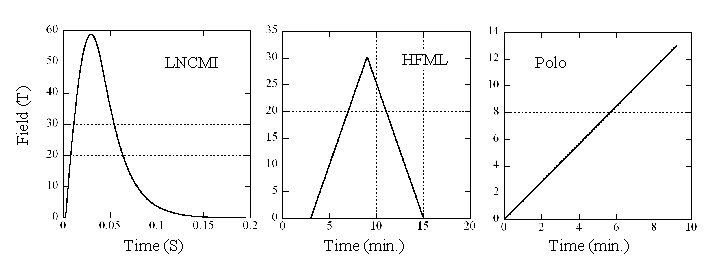
\includegraphics[scale=0.9]{Chapter-ExperimentalTechnique/Figures/ComparisonFieldSweeps/ComparisonFieldSweeps}
        \caption{From left to right: Typical field sweep profiles for a pulse at the \ac{LNCMI}, Toulouse, a continuous positive sweep at the \ac{HFML}, Nijmegen and single positive upsweep for the Polo magnet, Bristol.}
        \label{Fig:Exp:ComparisonFieldSweeps}
    \end{center}
\end{figure}
For the longer sweeps such as the Nijmegen data sets, an additional offset was applied to the measurement which is proportional to the temperature as detailed below,
\begin{equation}
    R_{\textrm{corr.}} = R_{\textrm{meas.}} + F(T_{\textrm{base}} - T_{\textrm{meas.}})
\end{equation}
where $R_{\textrm{corr.}}$ is the corrected resistance, $R_{\textrm{meas.}}$ is the measured resistance, $T_{\textrm{base}}$ is the temperature that the temperature that the resistance values are converged towards and $F$ is an empirical scaling factor that brings the upsweep and downsweep data into line. The empirical factor was determined by inspection using the following method.
\begin{enumerate}
\item Take data where there is a clear component that is due to the temperature drift and find the appropriate factor so that it disappears. Take these data as reference benchmarks.
\item Where the temperature component is not so clear, use the reference data and make an informed estimate of the factor based on resistance vs. temperature curves in zero field and \unit{13}{\tesla}
\end{enumerate}
The same factor is applied to both the positive and negative sweeps to avoid introducing artificialities into the Hall gradient. For the Polo data the temperature control was such that no correction was necessary.

\subsubsection{Field lag correction}

The Polo magnet has no sensor to measure field at the sample, with the field values being calculated from the power supply current. In the data there is evident hysteresis in all sweeps and is illustrated in figure~\ref{Fig:Exp:PoloHysteresis} which suggests that the actual field lags slightly behind the indicated field possibly due to induction effects in the magnet coil and/or the power supply. To correct for this, the upsweeps and downsweeps were shifted towards each other until they overlapped, typically each by around \unit{0.2}{\tesla}. Any values which were corrected to less than \unit{0}{\tesla} or more than \unit{13}{\tesla} were then not used in the analysis.
\begin{figure}[htbp]
    \begin{center}
        \includegraphics[scale=1.1]{Chapter-ExperimentalTechnique/Figures/PoloHysteresis/PoloHysteresis}
        \caption{An example of the measured voltage of separate up and downsweeps which demonstrate the lag in actual field compared to the indicated field.}
        \label{Fig:Exp:PoloHysteresis}
    \end{center}
\end{figure}

\subsubsection{Combining up and downsweeps}

For all the data values there is an upsweep portion and a downsweep portion which overlap and are averaged together to reduce noise. However many portions of data have regions which drift due to changes in the out-of-phase component or anomalies such as spikes and so in these cases the regions are recorded in a configuration file and the scripts that combine the sweeps ignore the problem regions and instead use data from the counterpart sweep in isolation. Similarly, when hysteresis is encountered in the pulsed data, by convention the upsweep is ignored since it is more rapid than the downsweep which generally results in more spikes and out of phase problems.

To obtain the Hall and \ac{MR} components using equation~\ref{Eqn:Exp:HallMRExtraction} we need to obtain comparable data points with shared field values. To do this one of two technique was employed. For the high-field data, this is done by binning the data and taking the average of the values in each of the bins so that they share the same field values. The data taken from the Polo magnet is linearly interpolated to a predefined set of field values.

\subsubsection{Linear fits to Hall data}

Hall data for all samples were fitted using a standard linear least squares fit which was performed using Python for the Polo data and Delphi for the high-field data due to the different preprocessing requirements described in the previous section. A cutoff is specified so that only the data above the cutoff is fitted in the region where the linear behaviour is recovered. The cutoff value is found by inspection of the Hall data with reference to the \ac{MR} component. The precise point where linear behaviour is recovered is not always clear and so two cutoffs were specified which defined the upper and lower bounds for the start of the linear region. The limits contribute to the error in the Hall gradient with the final gradient being taken as the average of the fits from the two cutoff limits.

\subsubsection{Normalising the high field data}

The Polo data was taken in the Hall configuration and so corresponds to the true Hall voltage, whereas the data from the first visit to the \ac{LNCMI} was on sample measured in the \ac{MR} configuration and so represent some unknown fraction of the true Hall voltage. Moreover, the rest of the high field data was taken in the diagonal configuration meaning the voltage path was over a different portion of the sample to the Hall measurement which again means the Hall voltage is scaled by some factor. For these reasons the Polo magnet measurements were taken as the canonical absolute values for the Hall data, with the high field data scaled so that concurrent data at higher fields aligned, this process along with the variation between fits using the two different cutoff bounds define the error bars in the data.


\subsection{Determining the doping}

Three techniques have been identified for determining the doping for this thesis. The most simple and well known method for determining the doping of a material utilises the so-called `universal' Tallon relation~\cite{Presland1991} which links $T_c/T_c(\textrm{max})$ to $p$ as follows,
\begin{equation}
\label{Eqn:ExpH:TallonRelation}
T_c/T_c(\textrm{max}) = 1 - 82.6 (p - 0.16)^2
\end{equation}
This relation was established based on measurements of \acf{LSCO} which exploit the direct relation between Sr content and the doping (assuming stoichiometric oxygen).

The second technique, particular to \ac{BSCO}, was published by Ando \etal~\cite{Ando2000} in 2000 where samples of \ac{BSCO} were compared with Hall measurements of other cuprates where the carrier concentration is more easily determined, in particular \ac{LSCO} was used again. The results lead to a very different relation between $T_c/T_c{\textrm{max}}$ which confined superconducting samples to a much narrower range of dopings\footnote{The justification being that increasing disorder suppressed $T_c$ as you move away from optimal doping.} and is given by the following relation,
\begin{equation}
\label{Eqn:Exp:AndoRelation}
T_c/T_c(\textrm{max}) = 1 - 254.3 (p - 0.16)^2
\end{equation}
which was extracted from the Ando paper based on dopings determined by La concentrations. 

There is however some doubt as to whether it is appropriate to compare \ac{LSCO} and \ac{BSCO} measurements across the superconducting dome, especially with regards to Hall measurements, given the proximity of the van-Hove singularity in \ac{LSCO} which should lead to a depression in the apparent carrier density above $p=0.18$.

The final technique is by comparing instead \ac{BSCO} and \ac{TL2201} which have very similar structures, and van-Hove singularities at much higher doping than \ac{LSCO}\footnote{\ac{TL2201} has a van-Hove singularity at a much higher doping than even \ac{BSCO}. At $p=0.26$ (or rather $p=1.26$), \ac{ARPES} measurements have shown the van-Hove singularity in \ac{TL2201} lies a few \unit{eV} below the Fermi energy~\cite{Plate2005}.} . Doping in \ac{TL2201} has been well characterised in the overdoped side through recent \ac{dHvA} experiments~\cite{Bangura2010} which maps well to where the majority of our \ac{BSCO} samples lie. Here the doping is determined using the Tallon relation for underdoped to slightly overdoped samples with $T_c/T_c(\textrm{max})$ down to $0.71$, below this value a linear relation is used: $T_c/T_c(\textrm{max}) = 2.390 - 7.696p$. Again some a priori knowledge of the approximate location (i.e. overdoped or underdoped) on the superconducting dome is required and further investigation may be required to determine which side of the dome a sample lies.

